\section{local systems on natural alternating diagrams}

Suppose we have a positive braid word $\omega$ then we have the associated natural alternating diagram $(M, \Lambda'_0, \Lambda'_\infty)$ defined in the previous section.

We can associate a quiver $Q$ to the alternating diagram in such a way that

\begin{itemize}
\item we have one vertex for regions where all hairs are pointing outward/inward
\item for each crossing, we have an arrow from the vertex corresponding to the region where all hairs pointing outward to inward
\end{itemize}

For example, for each generator region of a natural alternating strand diagram:

\begin{figure}[H] 
    \centering
    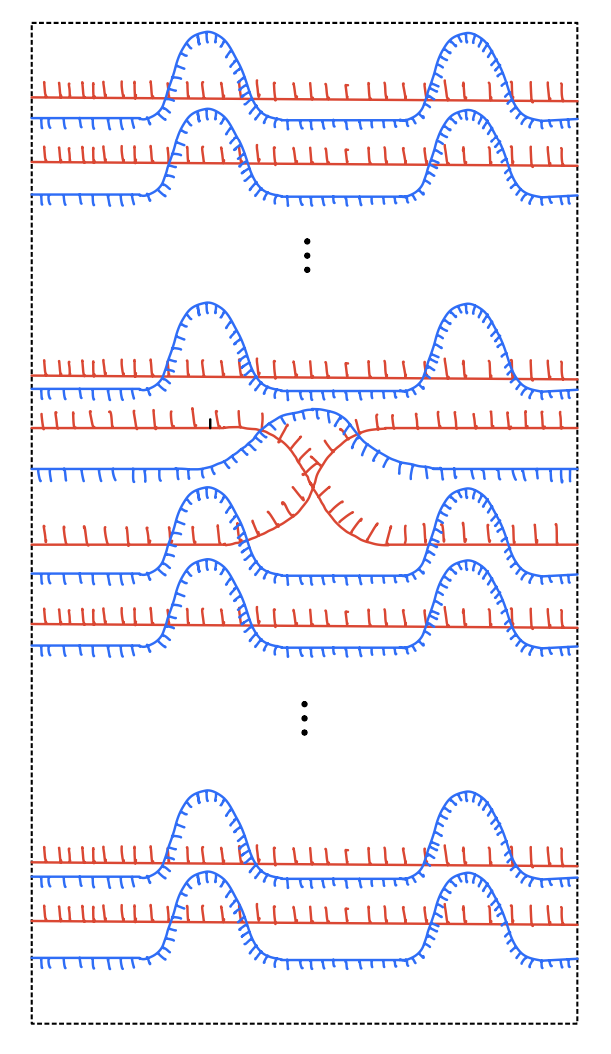
\includegraphics[scale = 0.95]{diagrams/local_systems_on_as_diagrams/1-1.png} 
    \caption{Your caption here}
    \label{fig:your-label}
\end{figure}

we have the following associated quiver:

\begin{figure}[H] 
    \centering
    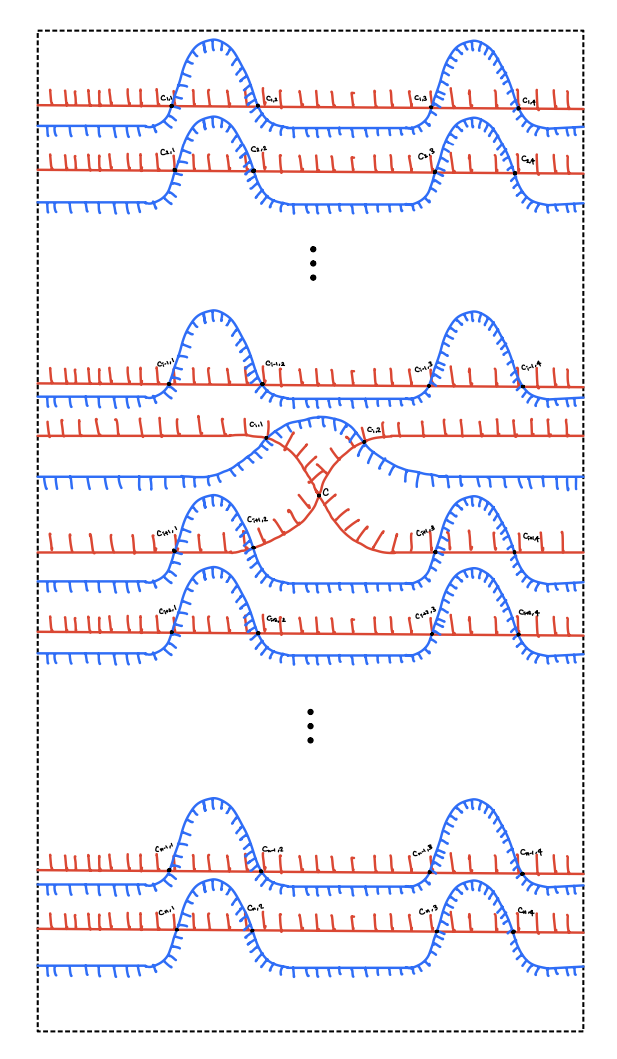
\includegraphics[scale = 0.95]{diagrams/local_systems_on_as_diagrams/1-2.png} 
    \caption{Your caption here}
    \label{fig:your-label}
\end{figure}

Once we have an alternating strand diagram, we have the associated conjugate surface $S_{conj}$. Furthermore, we can embed the underlying undirected graph of the quiver $Q$ in $S_{conj}$ in such a way that $S_{conj}$ deformation retracts to $Q$(with abuse of notation I will denote this underlying undirected graph as $Q$)(STZ??)
Suppose we have a rank $1$ local system on the conjugate surface associated with $(M, \Lambda'_0, \Lambda'_\infty)$, then restricting to $Q$, we get a local system on $Q$. Note that the pullback, induced by the restriction map, between the space of local systems $H^1(S_{conj}, \C^*) \rightarrow  H^1(Q,\C^*)$ is an isomorphism.

$H^1(Q,\mathbb{C}^*)$ is isomorphic to $(\C^*)^{|Arr(Q)|}//(\C^*)^{|Vert(Q)|}$
here the group action is defined as the following : let $g_v \in (\C^*)^{|Vert(Q)|}$
(more precisely, $g_v := (g^{\delta_{w,v}})_{w \in Vert(Q)}$ where $\delta$ is the Kronecker delta),
then $g_v \cdot (x_a)_{a\in Arr(Q)}$ is 

\begin{itemize}
\item for entries with index $a$ such that the source of $a$ is $v$ i.e. $s(a) = v$, we have $g_v \cdot x_a$
\item for entries with index $a$ such that the target of $a$ is $v$ i.e. $t(a) = v$, we have $g_v^{-1} \cdot x_a$
\end{itemize}


Now we define the associated constructible sheaf on some regular cell complex refinement of the natural alternating strand diagram associated with a rank $1$ local systems on $Q$.

First, I will describe the special kind of regular cell complex associated with the alternating strand diagram called the regular cell complex refinement of the natural alternating strand diagram. I will define the refinement for each generator region and glue them to get the global regular cell complex.

\begin{definition}
Suppose we fix a generator region for the alternating strand diagram. Then we denote the $j^{th}$ crossing(numbering starts from left to right) the $i^{th}$ blue strand(numbering starts from top to bottom) crosses red strands as $c_{i,j}$. We will call the crossing between $i^{th}$ and $i+1^{th}$ red strand as $c$.

For each crossing $c_{i,j}$ we add 

\begin{itemize}
\item two $0$ dimensional strata at the interiors of the $1$ dimensional strata at the northwest(northeast resp.) and southwest(southeast resp.) of the crossing when $j$ is even(odd resp.). Note these $0$ dimensional strata splits the original $1$ dimensional strata i.e. $NW$($NE$ resp.) and $SW$($SE$ resp.) into two $1$ dimensional strata $NW_1,NW_2$($NE_1,NE_2$ resp.) and $SW_1,SW_2$($SE_1,SE_2$ resp.).
\item one $1$ dimensional stratum at the interior of the west region of the crossing connecting the above two $0$ dimensional strata. 
\end{itemize}

We will draw this line in a squiggly line. Also for the crossing $c$, we add

\begin{itemize}
\item two $0$ dimensional strata at the interiors of the $1$ dimensional strata at the northwest and southwest of the crossing.
\end{itemize}

We give co-orientations so that the hairs are pointing toward the crossings.
 
Below is the picture of a generator region of a natural alternating diagram:

\begin{figure}[H] 
    \centering
    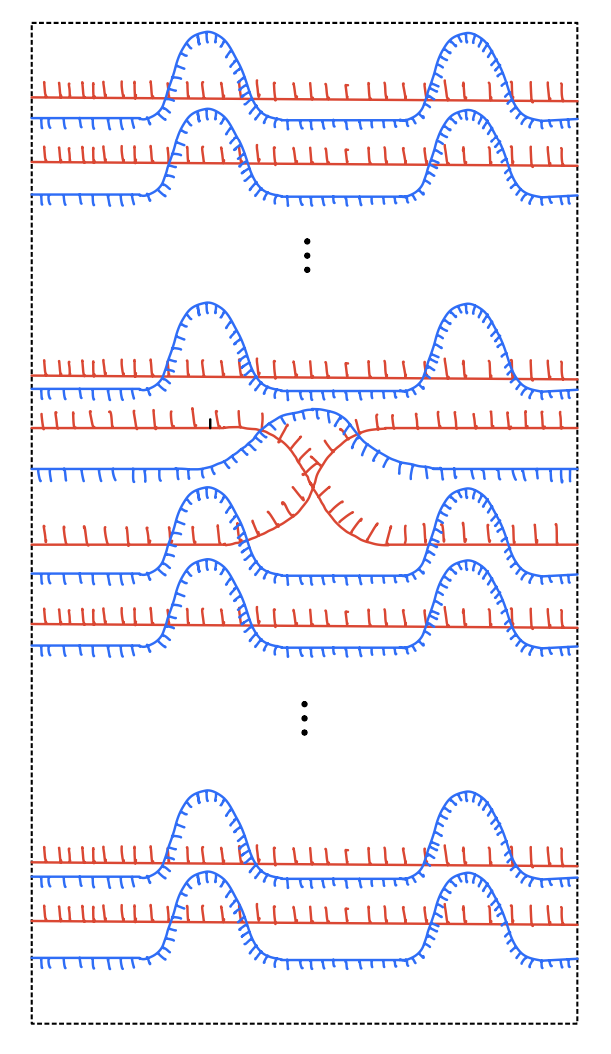
\includegraphics[scale = 0.95]{diagrams/local_systems_on_as_diagrams/2-1.png} 
    \caption{Your caption here}
    \label{fig:your-label}
\end{figure}

Below is the picture of a generator region of a natural alternating diagram with the crossings labeled(cannot see the labels clearly!):

\begin{figure}[H] 
    \centering
    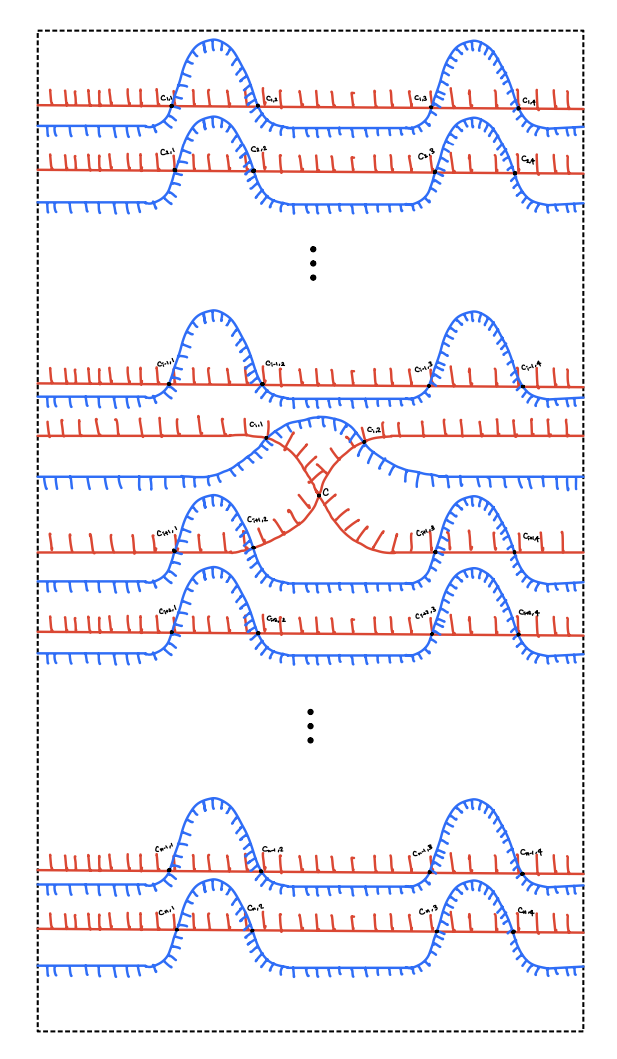
\includegraphics[scale = 0.95]{diagrams/local_systems_on_as_diagrams/2-2.png} 
    \caption{Your caption here}
    \label{fig:your-label}
\end{figure}

Below is the picture of the regular cell complex refinement in a generator region:

\begin{figure}[H] 
    \centering
    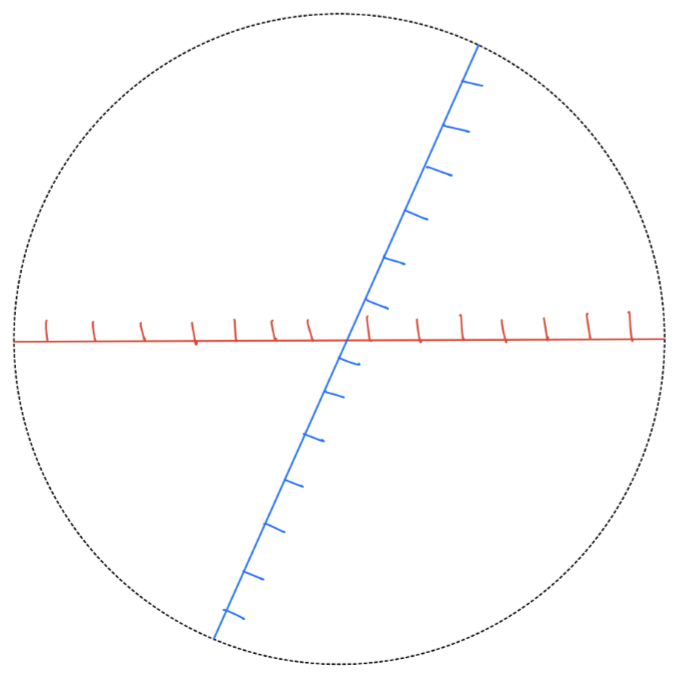
\includegraphics[scale = 0.95]{diagrams/local_systems_on_as_diagrams/3.png}
    \caption{Your caption here}
    \label{fig:your-label}
\end{figure}
\end{definition}

Now I will describe a way to specify a constructible sheaf on the above regular cell complex refinement associated with the local system on $Q$. 

\begin{definition}
Suppose we have a local system on $Q$ which can be represented as an element $(x_A)_{a\in Arr(Q)}(\mathbb{C}^*)^{|Arr(Q)|}$:

\begin{enumerate}[label= (\roman*)]
\item stalk of the region where all the hairs are pointing outward is $\mathbb{C}[-1]$

\item stalk of the region where all the hairs are pointing inward is $\mathbb{C}$

\item stalk of the region that has crossing at its boundary and surrounded by a squiggly line is $\mathbb{C}\rightarrow\mathbb{C}$ where the map is multiplication by $x_a$ where $a$ is the arrow goes from the south of the crossing to the north of the crossing

\item the only nonzero genrization maps are region of type (\Rn{3}) to (\Rn{1}) or (\Rn{1}) to (\Rn{2})
\end{enumerate}

The map from (\Rn{3}) to (\Rn{1}) is
\[
  \begin{tikzcd}
    \mathbb{C} \arrow{r}{id} & \mathbb{C} \\
    \mathbb{C}\arrow{u}{} \arrow{r}{}& 0\arrow{u}{}
  \end{tikzcd}
\]

The map from (\Rn{1}) to (\Rn{2}) is 
\[
  \begin{tikzcd}
	0 \arrow{r}{} & \mathbb{C} \\
    \mathbb{C}\arrow{u}{} \arrow{r}{id}& \mathbb{C}\arrow{u}{}
  \end{tikzcd}
\]
\end{definition}

Note that the group action maps a constructible sheaf to the isomorphic constructible sheaf. Therefore, we have a well-defined map
$H^1(S_{conj},\mathbb{C}^*)\rightarrow \mathcal{M}_1((M,\Lambda'_0,\Lambda'_\infty, \Lambda'_{squig}))$ where $\Lambda'_{squig} = (\Phi'_{squig}, \xi'_{squig})$ is the squiggly lines and it's co-orientations in the regular cell complex refinement of the natural alternating diagram.